\documentclass[
	%a4paper, % Use A4 paper size
	letterpaper, % Use US letter paper size
]{jdf}


\author{Shashvat Sinha}
\email{shashvat.sinha@gatech.edu}
\title{Assignment M2 (Summer 2020)\\CS6750}

\begin{document}
%\lsstyle

\maketitle

\begin{abstract}
    For my \textbf{M*} assignments in CS6750 (Summer 2020), I have chosen to redesign the interface that \textbf{LinkedIn} uses for its messaging. There are several aspects of the messaging interface that, in my opinion, could be improved - there is limited support for threading, messages do not support rich text, and the editor is geared towards short texts rather than a proper messaging platform. 
    
    As a networking tool LinkedIn would benefit from improved communication between its users, as it would improve the value proposition its users see. By the end of the M* assignments, I plan to focus on the task of communicating using LinkedIn messaging, taking it  through a complete design lifecycle. 
\end{abstract}

\section{Needfinding Execution}
We performed the following NeedFinding executions:

\begin{itemize}
    \item Analysis of product reviews
    \item Participant observation
    \item Evaluation of existing user interfaces
\end{itemize}

Based on what we learnt in the needfinding via product reviews and participant observation,  exercised the alternative option described in \textbf{\emph{M1}}, the evaluation of existing user interfaces.


\subsection{Execution A: Analysis of Product Reviews}
\subsubsection{Overview}
A generic search on LinkedIn and LinkedIn messaging returned results of articles which were predominantly geared to how people were using LinkedIn, e.g. recruiters and marketers spamming users inboxes, rather than critiques of LinkedIn itself.

Further analysis and curation yielded the following reporting and reviews of the LinkedIn messaging redesigns in 2015 and 2017 that moved from email style messaging towards shorter chat style messaging.

\begin{table}[h] % [h] forces the table to be output where it is defined in the code (it suppresses floating)
	\caption{Analysis of Product Reviews}
	\small % Reduce font size
	\centering % Centre the table
	\begin{tabular}{L{0.25\linewidth} C{0.05\linewidth} L{0.15\linewidth} L{0.13\linewidth}  L{0.4\linewidth}}
		\textbf{Theme} & \textbf{Score} & \textbf{Citation} & \textbf{Review Date} & \textbf{Remarks}\\
		\toprule[0.5pt]
		Messaging interface redesign to favor short messages & 2 & \cite{hull_2015} & Sep 2015 & Reviewer goes through LinkedIn's (then) new messaging interface and gives it poor marks for execution.\\
		\midrule
		Walkthrough of LI's short messages & 4 & \cite{simos_2018} & Jul 2018 & Reviewer has positive view on LinkedIn short messaging\\
		\midrule
		Contact and messaging tags & 1 & \cite{driskell_2017} & Apr 2017 & User is unhappy with removal of message and contact tagging facility, describes how to leave LinkedIn\\
		\midrule
		LinkedIn's Facebook style messaging & 4 & \cite{gonzalez_2017} & Jun 2017 & Reviewer has positive view on LinkedIn short messaging, comparing it to Facebook's\\
		\midrule
		LinkedIn's messaging is now FB/Hangout style & 3 & \cite{ingraham_2020} & Feb 2020 & Reviewer describes how LinkedIn is now more like Facebook and Hangouts\\
		\midrule
		LinkedIn's messaging is now on the main page & 3 & \cite{lunden_2017} & Jan 2017 & Reviewer describes how chat is now on the main page to keep the user's attention on another feature, the news feed\\
		\midrule
		Walkthrough of LI's short messages & 4 & \cite{price_2017} & Apr 2017 & Messaging is designed to be everywhere on the LI interface instead of in its own tab\\
		\midrule
		Messaging on every page & 3 & \cite{warren_2017} & Jan 2017 & Messaging is on every page instead of on its own, similar to Facebook\\
		\midrule
		
	\end{tabular}
\end{table}

\subsubsection{Analysis}

The general themes are:
\begin{itemize}
    \item LinkedIn has moved from email style messaging to Facebook/Hangouts style short messages. 
    \item This move brings LinkedIn in line with its social networking peers.
    \item A second redesign also moves LinkedIn's messaging from its own page to all over the LinkedIn website, so that users can carry out their chat anywhere. This is a copy of Facebook's chat functionality.
\end{itemize}


\begin{enumerate}
    \item What kind of user has written the opinion or review.
    All but three reviews seem are written by staff writers for major online publications. In two cases the writers wrote on LinkedIn's own blog website. One case was of a user who wrote on their own website - this user was the most dissatisfied with the redesign.
    \item From what lens does the writer view LinkedIn - do they consider it a networking tool, a recruitment tool, or something else? 
    The reviews are written from a point of view where LinkedIn is considered a social networking tool, where its peer is Facebook.
    \item What is the writer attempting to do with LinkedIn? Is it related to the messaging capability?
    As staff writers, the reviewers (except one) are merely reporting the release of new features, rather that actually try to use LinkedIn as a service. There was only one exception to this (\cite{driskell_2017}), who found the redesign so detrimental to his productivity, he described how to migrate away from LinkedIn.
    
    \item What is the writer failing to do? Is there a Gulf of Execution and Gulf of Evaluation we can identify?
    The one writer who did have an open critique (\cite{driskell_2017}) had a clear Gulf of Execution, which could not be bridged after the redesign.
    
    \item What, if any, suggestions does the writer make as a means to make them whole again?
    The only writer with a critique (\cite{driskell_2017}) would have wanted LinkedIn's messaging to regain its tagging feature.
\end{enumerate}

\subsubsection{Conclusion}
The needfinding approach of \textbf{analysis of product reviews} did not return useful data.
There were very few actual product reviews that I was able to find of LinkedIn. The vast majority were critiques of LinkedIn's user culture and behavior, which does not help our exercise. The others were PR pieces written by staff writers who seemed to all say the same few things (e.g. comparisons with Facebook, the availability of messaging on all LinkedIn pages)

I would consider this needfinding approach for this topic to be sub-optimal.

\subsection{Execution B: Participant Observation}
\subsubsection{Overview}

I am a user of LinkedIn. Over the years, I have made several observations about LinkedIn's messaging system as I tried to use it for tasks related to networking and communication.

In this section I will evaluate these observations through a needfinding lens.

%My initial plan was to take the outputs of the previous step - the Analysis of Product Reviews - and try to visit those experiences on myself. 

%The analysis indicated that the vast majority of LinkedIn reviews were not in fact critical objective assessments, but were in fact public relations pieces posted by staff writers for industry publications. The other category of reviews were user guides with the existing paradigm and user interface, which did not make an attempt to reimagine the concept of business network messaging.

%While this may seem like a setback, one must consider that this also indicates that there is an \textit{\textbf{unmet need}} for a critical evaluation and open rethinking of the interface.


\subsubsection{Analysis}
\textbf{Note on bias:} I attempted to mitigate the effects of \textit{confirmation bias} by splitting my Participant Observation exercise into two parts. The first part, where I put down my observations, was done \textit{before} the analysis of product reviews.

The second part, where I try to visit the experiences of reviewers, and try them out myself was to be done \textit{after} I completed the analysis of product reviews.

These are my observations about LinkedIn messaging, and the issues I felt needed to be addressed:
\begin{enumerate}
    \item \textbf{Observation}: LinkedIn messaging is not specifically part of a particular screen or tab, but is instead spread all over the interface on every screen.
    \begin{enumerate}
    \item\textbf{Issue}: If you want to message someone, it is not conceptually clear how to start it off - since there is no well defined starting point.
    
    \item\textbf{Issue}: The messaging windows overlay and obscure the other parts of the interface.
         
    \end{enumerate}

    \item \textbf{Observation}: Messages to a person show up in a small overlay window.

    \begin{enumerate}
    \item\textbf{Issue}: It is difficult to edit and in general compose a useful mail type long form communication in a small window. I often get messages asking for my mail address so that a proper discussion can happen outside the LinkedIn interface.
    
    \item\textbf{Issues}: The small overlay windows can't be moved or sorted to organize in a manner of your choosing.
    \end{enumerate}
    \item \textbf{Observation}: There is no obvious threading, grouping or theme organisation for the messages. 
    
    \begin{enumerate}
    \item\textbf{Issue}: Is it impossible to use LinkedIn's interface for managing a messasing theme (e.g. one theme could be networking, another could be applying for a specific job).
    \end{enumerate}
\end{enumerate}


\subsubsection{Conclusion}
The design of LinkedIn messaging as a short message texting service in the form of Facebook is limits the functionality that I as a participant believe could be part of LinkedIn.

The functionality could be enriched by making messaging central or at least pivotal to the platform, rather than an overlay over other features.

\subsection{Execution C: Evaluation of Existing User Interfaces}

\subsubsection{Overview}
There are several Personal Relationship Management (PRM) alternatives to LinkedIn, as well as examples from the CRM world. Given below is my research and analysis on their features and abilities.

\subsubsection{Analysis}
The following are the alternative platforms I explored:

\begin{table}[h] % [h] forces the table to be output where it is defined in the code (it suppresses floating)
	\caption{Existing User Interfaces}
	\small % Reduce font size
	\centering % Centre the table
	\begin{tabular}{L{0.2\linewidth} L{0.25\linewidth} L{0.45\linewidth}}
		\textbf{Application/Site} & \textbf{Link} & \textbf{Description}\\
		\toprule[0.5pt]
		Circles/ZooWho & \url{https://zoowho.com} & Relationship management, network management with email capability.\\
		\midrule
		Cloze & \url{https://www.cloze.com} & Relationship management, "Business-Grade" email\\
		\midrule
	\end{tabular}
\end{table}


Both products bring in the concept of engaging with your network in targeted, scheduled ways, with deep contextual information tied to the messaging that you do with your users.

It is possible to look at a contact and determine what activities you engaged with them on, and to look at activities or projects, and then see which contacts you engaged with on that topic. Naturally, from either route, the user can drop in deep and explore, and send follow up messages.


\subsubsection{Conclusion}
There exists a category of applications that attempt to bring greater structure to the act of messaging and staying in touch with your network of contacts and business related persons.

Both of these application treat the messaging aspect as a full fledged activity, and have a rich interface for that messaging as can be seen in figures \ref{fig:cloze1} and \ref{fig:cloze2}.

\section{Data Inventory}
\subsection{Who are the users?}
The users are persons who a) are members of LinkedIn and b) have an interest in staying connected to their network of contact via messaging.
\subsection{Where are the users?}
The users are globally distributed. From the context of the user, they are either using LinkedIn at work or home from their computers, or on the move on their smartphones via the LinkedIn app. We have chosen to limit our scope to the desktop usage of these users.
\subsection{What is the context of the task?}
One can assume two contexts, mutually competing:
\begin{enumerate}
    \item That the user comes to the interface intending to start a conversation/initiate a message/respond to a message.
    \item That the user comes to the interface with another intention, for example applying for a job or looking for a lead to a business need, and turns towards the messaging feature to find that information (e.g. a prior conversation with a contact).
\end{enumerate}

\subsection{What are their goals?}
Their goals are broad - to use the messaging feature of LinkedIn to further their interests.

\subsection{What do they need?}
Considering the two contexts above, the users need:
\begin{enumerate}
    \item A quick and well defined way to get to the messaging sub-system, find the necessary contact or thread, and start writing a message.
    \item An easy way to mine prior conversations for information that would be useful to another task.
\end{enumerate}


\subsection{What are their tasks and subtasks?}
Considering the two contexts above, the users tasks are:
\begin{enumerate}
    \item Find a contact or thread, and compose a mail.
    \begin{enumerate}
        \item Search for contact or thread.
        \item Compose a mail to that contact, or pick up and continue the thread.
    \end{enumerate}
    \item Given a context or reference, find a thread or contact.

\end{enumerate}

\section{Defined Requirements}
We shall define our requirements to be \textbf{Specific and Evaluatable}. Therefore we will write them as user stories (\cite{cohn} et. al.).

\subsection{Functionality}
These are the requirements that we will address in subsequent M* assignments
\subsubsection{A well defined Messaging section}

\textbf{As a} user interested in sending a message to a LinkedIn contact

\textbf{I want to} be able to directly go to an interface in LinkedIn for messaging

\textbf{Such that} is it quick, easy and obvious how to send a message to a contact.

\subsubsection{A rich and mail-like messaging interface}

\textbf{As a} user composing a message to a LinkedIn contact

\textbf{I want to} be able to edit the message in a large window with rich text editing controls and standard ways to format text, attach files and edit the message.

\textbf{Such that} the act of sending a message to a contact can be done in a manner similar to my other mail-type communications channels, thus reducing the cognitive load.

\subsubsection{Context, thread and sender-recipient aware search}

\textbf{As a} user looking for a specific contact or message thread

\textbf{I want to} be able to search for messages based on context (e.g. tags, subjects, projects, dates), content and sender or recipient filtering.

\textbf{Such that} Such that it is easy to find prior messages an threads based on what I remember about them (e.g. find me mails send in 2018 on a a job in San Francisco sent to persons with the last name 'Cook' or 'Jobs').

\section{Continued Needfinding}
For continued needfinding, I would get back the exercise I identified in M1, that of surveys.

There, I would attempt to verify the null hypothesis that arises from my exercises above.

For reference, please see Appendix 6.1

\section{References}

\printbibliography[heading=none]

\section{Appendix}
\subsection{Screenshots}

\begin{figure}[h]
	\centering
	\frame{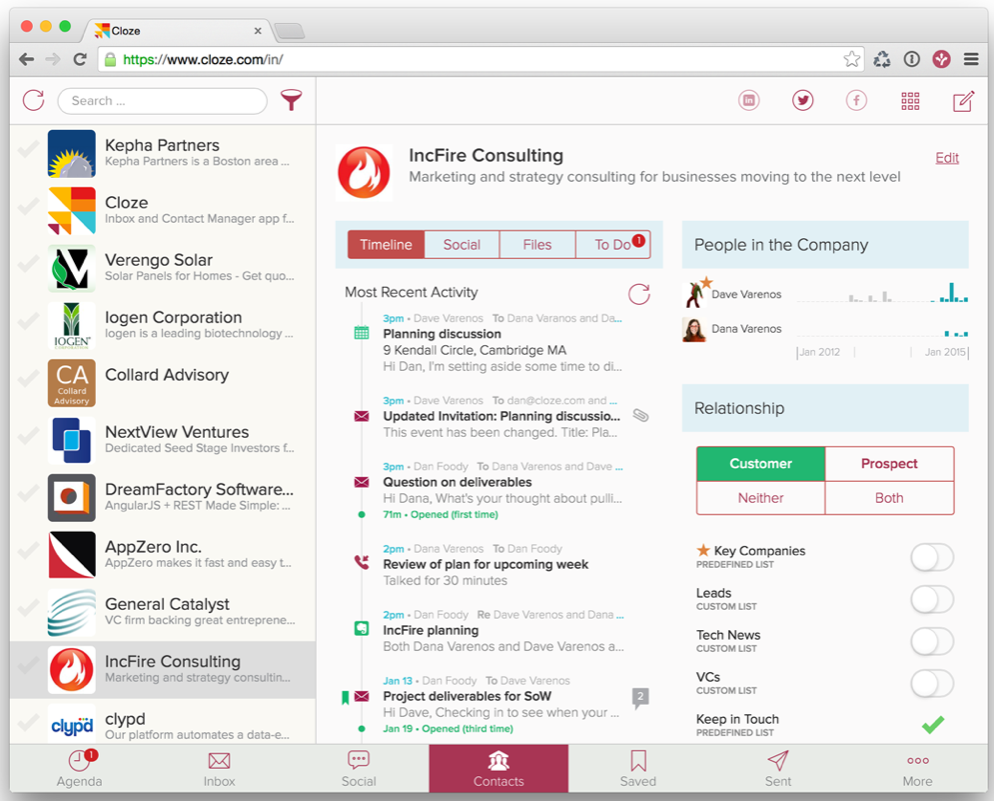
\includegraphics[width=7cm]{Figures/cloze1.png}}
	\caption{Cloze Messaging Context View}
	\label{fig:cloze1}
\end{figure}

\begin{figure}[h]
	\centering
	\frame{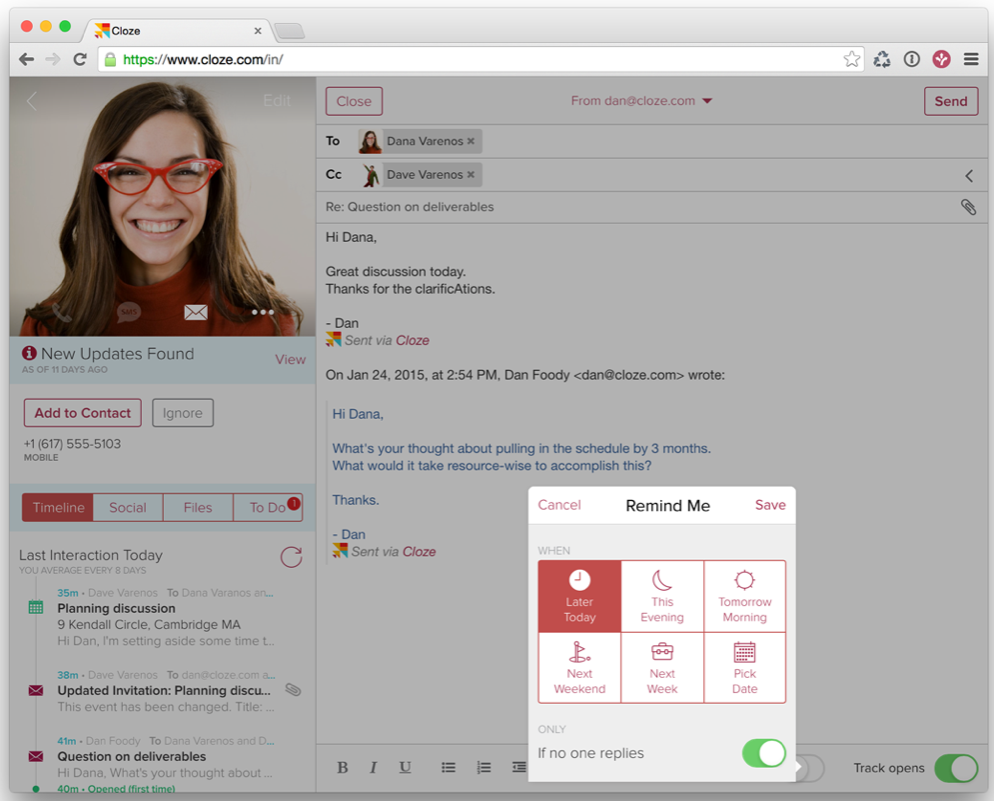
\includegraphics[width=7cm]{Figures/cloze2.png}}
	\caption{Cloze Messaging Compose View}
	\label{fig:cloze2}
\end{figure}


\subsection{Additional Needfinding (from M1)}
\textbf{I am quoting the alternate needfinding exercise I laid out in M1, that I could possibly use as part of further needfinding:}

\textbf{Plan C: Surveys}
LinkedIn is commonly used by fellow students, coworkers and friends \& family. All of them can be queried in a survey. Depending on LinkedIn's terms \& conditions of use, one may be able to post a survey on LinkedIn itself (e.g. using the wall post feature and take advantage of the network effect).

This survey will be informed by the exercise we did in Plan A above, namely finding the themes on improvement in LinkedIn's messaging that resonate with reviewers. We will attempt to determine if those themes resonate with our survey respondents. Care must be taken not to auto-suggest those themes to them, but to elicit responses that support or contradict the reviewers.

The questions would cover the following concepts (these are not the actual questions, as those would be determined from Plan A):
\begin{enumerate}
    \item Context of using LinkedIn
    \begin{enumerate}
        \item Where do you normally use LinkedIn?
        \item How often do you normally use LinkedIn?
        \item Is LinkedIn usage related to other events going on in your life (e.g. when you're dissatisfied with your current job).
    \end{enumerate}
    \item Goals or objectives driving the use of LinkedIn:
    \begin{enumerate}
        \item Why did you sign up for LinkedIn?
        \item Now that you are signed up, why do you actually visit LinkedIn?
        \item What do you do once you're on LinkedIn?
        \item What makes you leave the LinkedIn website?
    \end{enumerate}
\end{enumerate}

There are two biases that one should attempt to mitigate here:
\begin{itemize}
    \item Voluntary response bias - one can expect that persons responding to a voluntary survey may have extreme opinions about the product. The solution would be to have the survey be non-voluntary, by seeking to direct a specific set of users to respond to the survey regardless of their enthusiasm for the product.
    \item Observer bias - as the writer of the survey questions I would have to take care that my views and opinions do not color the survey questions. I do not have a solution for this, other than to be aware of this bias and make every attempt not to invoke it.
\end{itemize}



\end{document}